\section{Implementation and Application}

From the realistic rivers and oceans in the open world games to small water mechanism in puzzle games,
water is a common element of the background settings in many video games.
However, the types of object that could interact with water or the ways that they can do so in games are usually very limited.
Apart from the designs of the game, one big factor limiting the freedom of the interaction with water is on the technical side \cite{kellomaki2012water}.
Due to technical limitations, game developers lack the ways to fully simulate the water interactions and have to often manually overwrite the physical behaviors, which inevitably causes critical glitches \cite{RedditAssassin}.
With our method, game developers could arbitrarily put objects into water bodies without having to worry about physical glitches.

To apply our method into a game project, it is adviced to write a controller class for the water bodies, and let them be the source of the buoyancy forces;
doing so could avoid having to add a ``buoyancy force receiver'' on every single solid objects.
The water body controller does mainly two things:
\begin{enumerate}
	\item Maintain a collection of all solid objects that are submerged in this water body.
	\item Calculate and apply the forces contributed by the water body onto the objects in each physical frame.
\end{enumerate}

In each physical frame, the brief outline of the water body controller's tasks is given as Table \ref{water-controller-main-loop}.

\begin{table}[htb]
	\centering
	\begin{lstlisting}[style=pseudo]
		input sampleDensity
		input submergedBodies
		do in every physical frame
			foreach body in submergedBodies
				surfaceArea := CalculateSurfaceArea(body)
				sampleCount := surfaceArea * sampleDensity
				samples := SampleOverSurface(body, sampleCount)
				effects := new List
				add MakeBuoyancies(body, samples) to effects
				add MakeResistances(body, samples) to effects
				netEffect := $\bigoplus$ effects
				apply netEffect on body
			done
		done
	\end{lstlisting}
	\caption{The main loop of the water controller.}
	\label{water-controller-main-loop}
\end{table}

And the data type of the samples output by \texttt{SampleOverSurface} is defined as in Table \ref{surface-sample-data-def}.
Both the position and the normal vectors should in the world space instead of the physical bodie's local space, because that is where the calculations take place.

\begin{table}[htb]
	\centering
	\begin{lstlisting}[style=pseudo]
		datatype SurfaceSample
			position: Vector
			normal: Vector
			area: float
			weight: float
		end
	\end{lstlisting}
	\caption{The type definition for a sample on the surface.}
	\label{surface-sample-data-def}
\end{table}

It is important to feed the samples al at once in to the functions that compute the physical effects such as \texttt{MakeBuoyancies} and \texttt{MakeResistances}, since they need to accumulate the weights of the samples to normalize them before returning.

Table \ref{mesh-sampling-algorithm} gives an algorithm for generating random samples over a mesh.

\begin{table}[htb]
	\centering
	\begin{lstlisting}[style=pseudo]
		function SampleOverSurface
			input body
			input count
			vp := body.mesh.vertexPositions
			foreach i from 0 to count-1
				ti := random integer from 0 to body.mesh.triangleCount-1
				triangle := [vp[ti+0], vp[ti+1], vp[ti+2]]
				foreach position in triangle
					position = body.localToWorldMatrix * position
				done
				i = triangle[1] - triangle[0]
				j = triangle[2] - triangle[0]
				cross = i $\times$ j
				area = 0.5 $\times$ cross.magnitude
				yield new SurfaceSample {
					position = SampleInTriangle(triangle)
					normal = Normalize(cross)
					area = area
					weight = area
				}
			done
		end
	\end{lstlisting}
	\caption{The algorithm for generating random samples over a mesh.}
	\label{mesh-sampling-algorithm}
\end{table}

Figure \ref{boat-sample} shows an example of an application of our method.
A boat is floating on the sea; a pack of heavy balls are spawning above the boat and falling into it.
Without having to write any additional codes, just by keeping loading heavy balls onto the boat, the sunk depth of the boat automatically increases.

\begin{figure}[htb]
	\centering
	\begin{subcaptionblock}{0.46\textwidth}
		\centering
		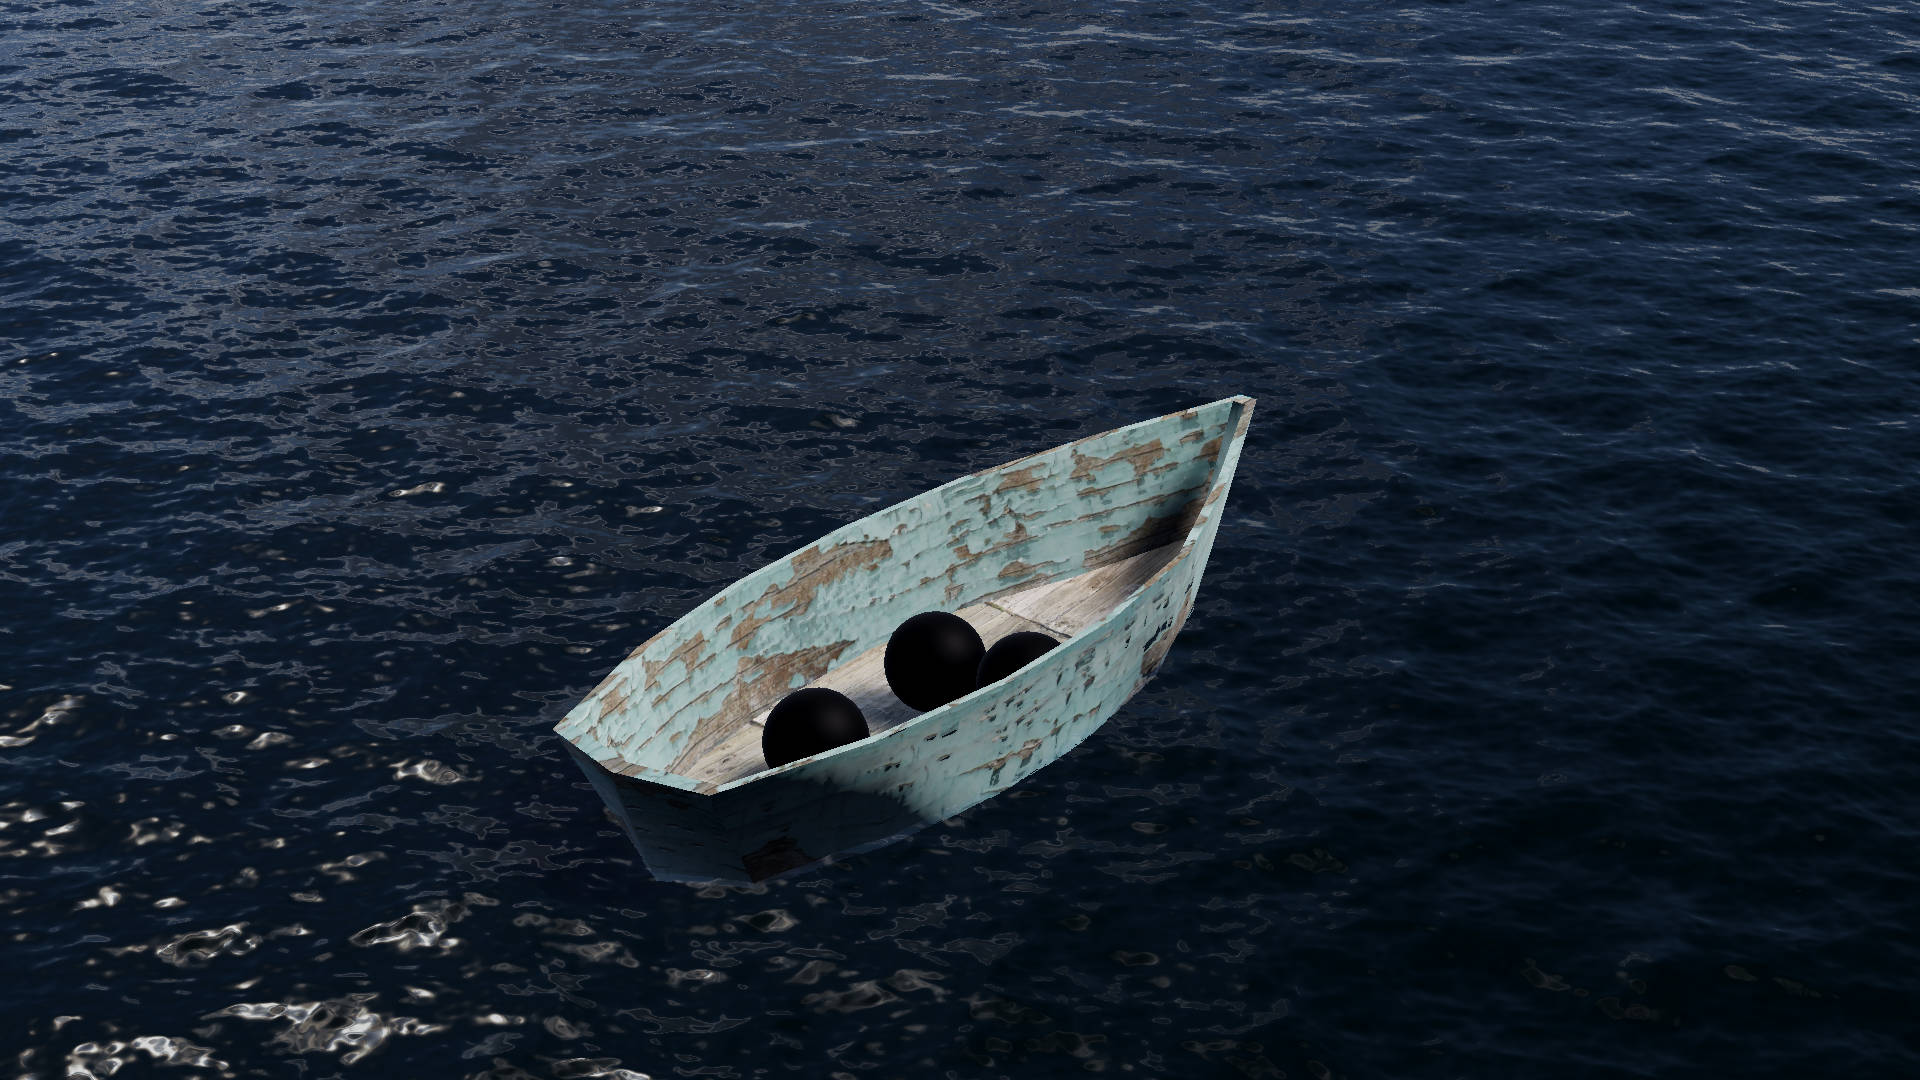
\includegraphics[width=0.9\textwidth]{figures/light-boat.jpg}
		\caption{A boat containing a few balls.}
	\end{subcaptionblock}
	\begin{subcaptionblock}{0.46\textwidth}
		\centering
		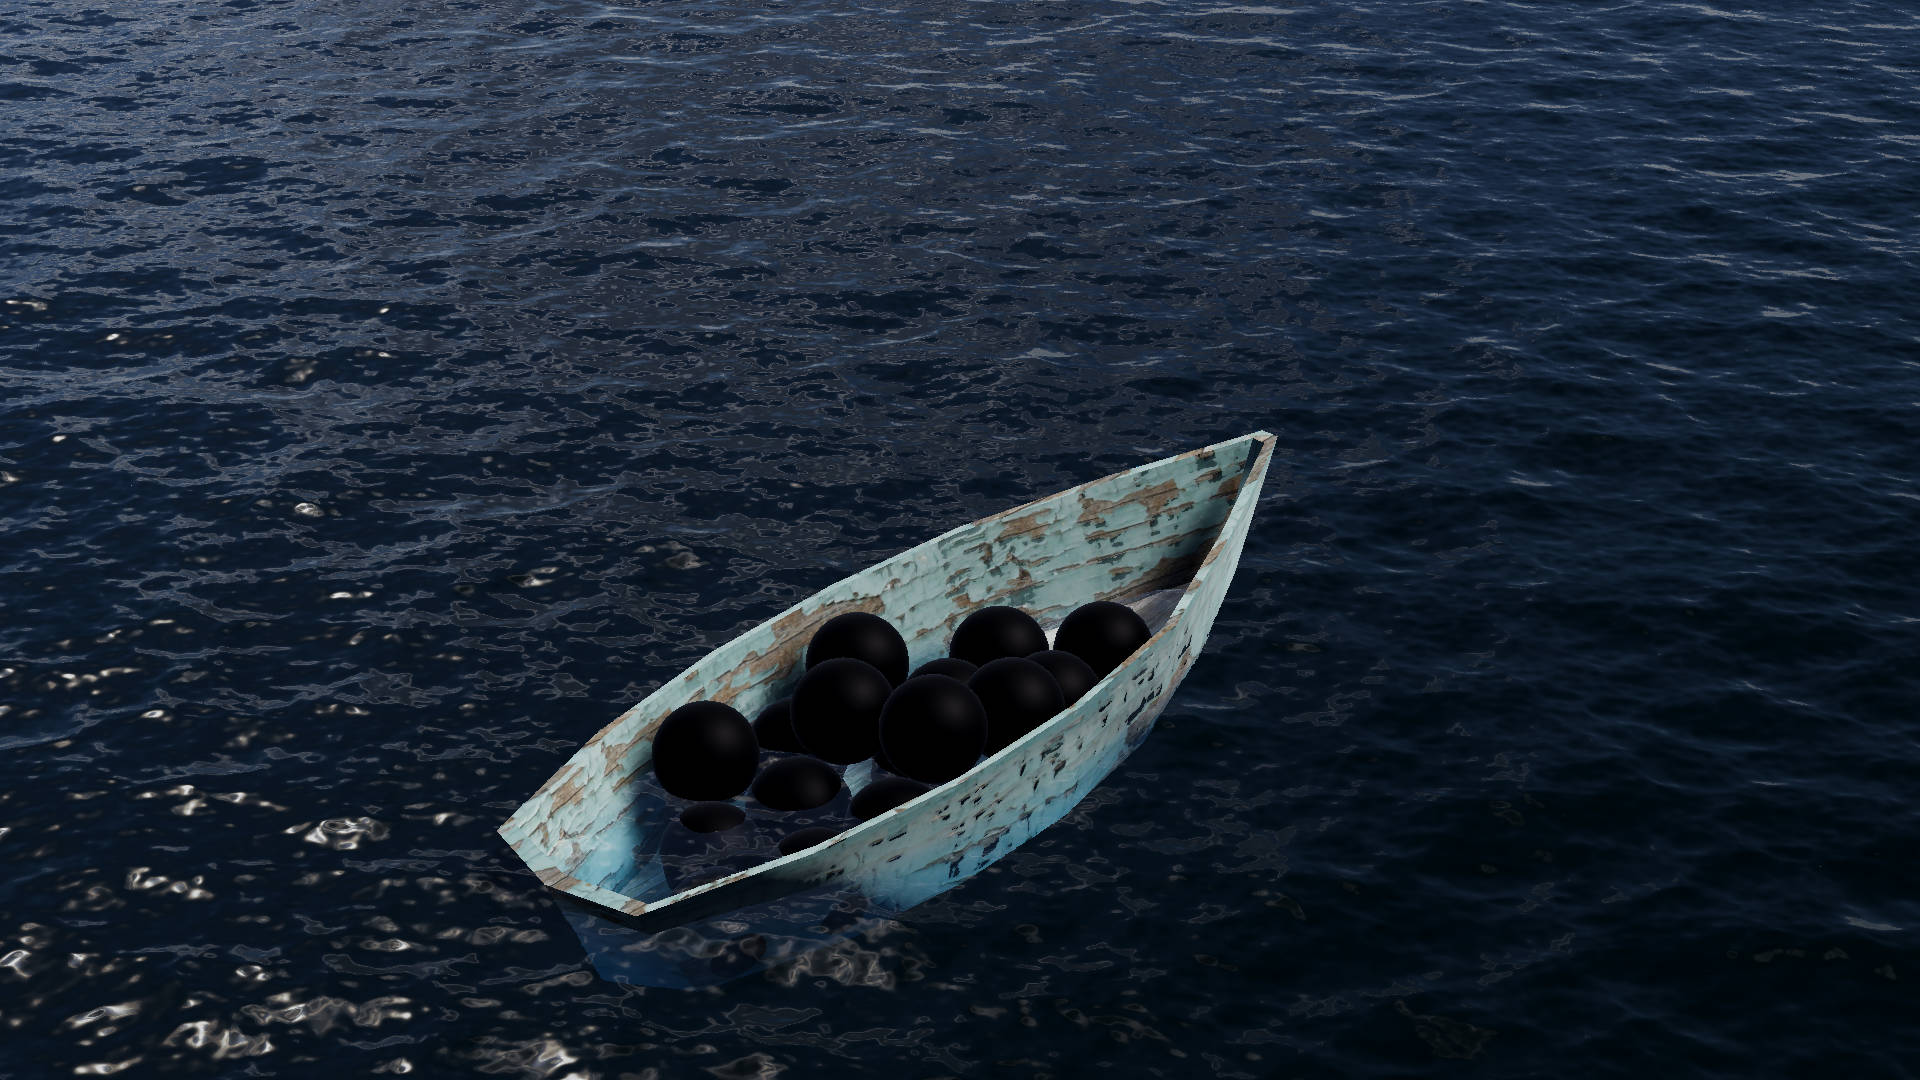
\includegraphics[width=0.9\textwidth]{figures/heavy-boat.jpg}
		\caption{The same boat containing many balls.}
	\end{subcaptionblock}
	\caption{Loading more balls onto the boat increases its depth.}
	\label{boat-sample}
\end{figure}

When applied in real game design, this extra freedom could allow game designers to create more complex mechanisms.
It is clear that often an open mechanism tends to lead to emergent behaviors \cite{sweetser2006emergent}, thus increasing the fun of the game.

Buoyancy simulation could also be used for creating the vibes.
Figure \ref{floating-donut-in-game} shows a screenshot of a poolcore-themed puzzle game, in which water is a main part of the visual design.
Adding objects that could float on water definitely helps emphasize the vibes of the pools.

\begin{figure}[ht]
	\centering
	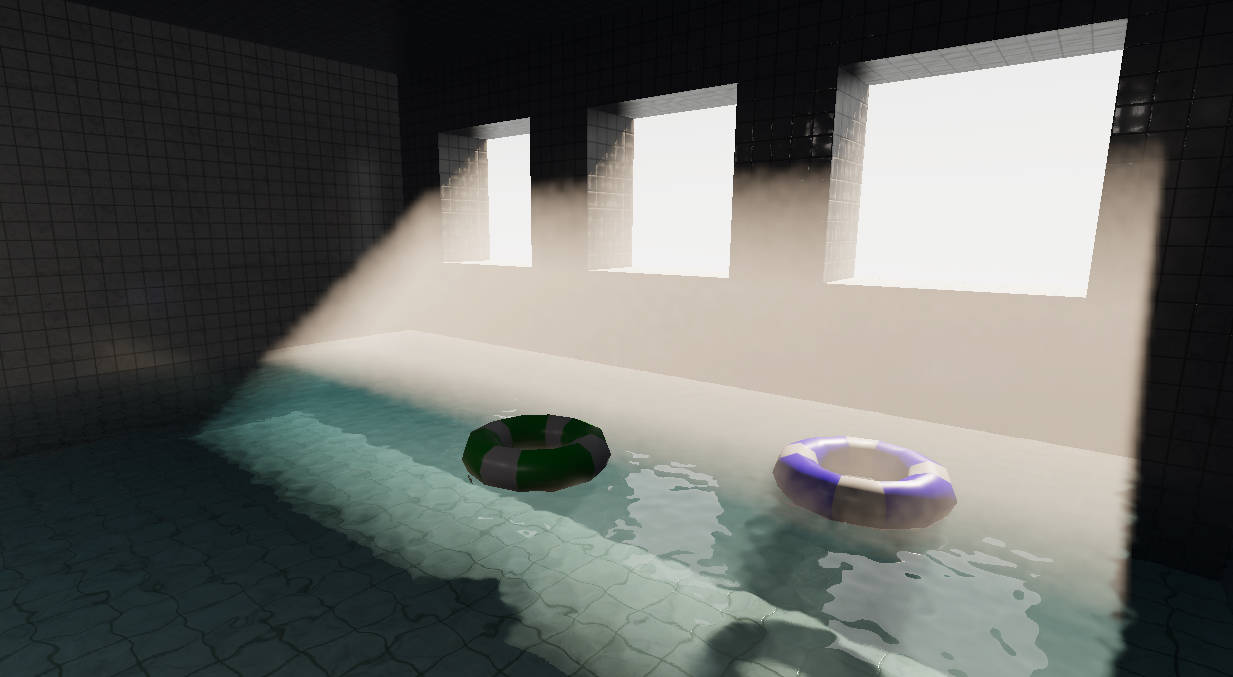
\includegraphics[width=0.4\textwidth]{figures/floating-donut-in-game.jpg}
	\caption{Floating objects can be seen in a poolcore-themed game.}
	\label{floating-donut-in-game}
\end{figure}